\documentclass{article}

% New commands declaration

\usepackage[frenchb]{babel}
\usepackage[T1]{fontenc}

\usepackage{natbib,bibentry}
\usepackage{color}
\usepackage{yfonts}
\usepackage{graphicx}
\usepackage{epsfig,subfigure}
\usepackage{amsmath,amssymb,amsfonts}
\usepackage{calc}

\usepackage{array}
\newcolumntype{L}[1]{>{\raggedright\let\newline\\\arraybackslash\hspace{0pt}}m{#1}}
\newcolumntype{C}[1]{>{\centering\let\newline\\\arraybackslash\hspace{0pt}}m{#1}}
\newcolumntype{R}[1]{>{\raggedleft\let\newline\\\arraybackslash\hspace{0pt}}m{#1}}


\DeclareGraphicsExtensions{.eps, .jpg, .png}

\parindent = 0mm

\bibliographystyle{plain}

\hoffset = -20mm
\voffset = -25mm
\textwidth = 160mm
\textheight = 240mm

\definecolor{lightgray}{gray}{0.2}


\newcommand{\expect}{{\rm I \mkern-2.5mu \nonscript\mkern-.5mu E}}
\newcommand{\equaldef}{\stackrel{d}{=}}
\newcommand{\argmax}{\operatornamewithlimits{argmax}}

\newcommand{\dnu}{16}
\newcommand{\solskip}{10mm}

\newcommand{\debutrep}[1]{\color{blue}\begin{center} \hrulefill \textbf{ #1 } \hrulefill \end{center} }
\newcommand{\finrep}{\vspace*{5mm}\hfill $\square$\color{black}\vspace*{5mm}}


\begin{document}

\baselineskip = 4mm
\title{Traitement des Signaux Aléatoires \\
Détection Quadratique}
\author{\textbf{4 ETI -- CPE Lyon }\\[3mm]
{Travaux Pratiques TSA}}
\date{2020-2021}

\maketitle

\noindent\fbox{
\parbox{\linewidth-2\fboxrule-2\fboxsep}
{ 
\vspace*{2mm}
{\large\bf Noms, Prénoms: }\\[3mm]
{\large\bf Groupe: }\\[3mm]
{\large\bf Date:}\\[2mm]}}
\vspace*{5mm}


\textbf{\Large Contexte et Objectif}\\[4mm]

On souhaite étudier expérimentalement la chaine de détection quadratique suivante:\\

\begin{center}
\includegraphics[width=0.9\columnwidth]{Chaine-Dq.png}
\end{center}

On souhaite détecter la présence ou non d'un signal aléatoire $S(t)$ dans un mélange signal $+$ bruit. Le signal $X(t)$ reçu est égal à:
$$
X(t) = S(t) + B(t) 
$$
Le signal $S(t)$ est un signal sinusoïdal de fréquence $\nu_0$, d'amplitude $A_0$, à phase équipartie sur $[0,2\pi[$ et modulé par un signal binaire $M(t) =  0$ ou $1$:
$$
S(t) = M(t) \cdot A_0 \cos (2\pi\nu_0 t + \phi) 
$$
Ce signal est bruité lors de la transmission par un bruit $B(t)$ gaussien, centré, stationnaire d'ordre 2 et de largeur de bande $B$ centrée sur $\nu_0$ (on supposera que le bruit est blanc sur le support fréquentiel du  filtre $\mathcal{F}_1$).
$$
X(t) = \left\{\begin{array}{ll}
B(t) & \mbox{si } M(t) = 0 ;\\[1mm]
A_0 \cos(2\pi\nu_0 t + \phi) + B(t) & \mbox{si } M(t) = 1
\end{array}
\right.
$$

L'objectif de la chaine de détection quadratique est de détecter dans l'observation reçue  $X(t)$, la présence ($\mathbf{M(t)=1}$) ou l'absence ($\mathbf{M(t) = 0}$) du signal utile $S(t)$.

\vspace*{5mm}

\textbf{ Etudier soigneusement le TD corrigé qui vous a été remis et qui détaille le calcul des rapports signal sur bruit (SNR)  aux différents étages de la chaine de détection. \\
Répondre aux questions de préparation qui suivent.
}

\paragraph{Question 1.}
On considère un bruit $B(t)$ centré, de puissance moyenne $\overline{P_B} = 5~V^2$.

Que mesure l'aire située sous la densité spectrale moyenne de puissance d'un bruit? \\
Que vaut cette quantité par rapport à l'écart-type, la variance, la moyenne du bruit? \\
Dans le cas du bruit $B(t)$ ci-dessus, calculer l'écart-type et l'amplitude $\Gamma_0$ de la densité spectrale.

\debutrep{réponse}

\finrep

\paragraph{Question 2.} 
On filtre le bruit $B(t)$ par un filtre passe-bande, de bande passante  $\Delta\nu$ centrée sur  la fréquence  $F_0$. 
Quel est le rôle du filtre passe-bande dans la chaine de détection quadratique. Sur quelle fréquence $F_0$ doit-il être accordé?

\debutrep{réponse}

\finrep

\paragraph{Question 3.} Soit $Y_B(t)$ la réponse du filtre $\mathcal{F}_1$ au bruit $B(t)$ ci-dessus. Que vaut la puissance de $Y_B(t)$ par rapport à celle de $B(t)$? Que vaut l'écart-type de $Y_B(t)$? \\
Application numérique avec $\Delta\nu = \dnu Hz$. \\

\debutrep{réponse}

\finrep

\paragraph{Question 4.}
A quoi sert l'ensemble {\sc quadrateur} $+$ {\sc filtre passe-bas RC}?

\debutrep{réponse}

\finrep

\paragraph{Question 5.}
Que signifie {\em hypothèse d'intégration forte} ? Quelle condition assure ici cette hypothèse?

\debutrep{réponse}

\finrep

 \paragraph{Question 6.}
Sous hypothèse d'intégration forte, que vaut  alors $\mathbb{E}\{W_B\}$? \\
Application numérique avec $B(t)$ et $\Delta\nu = \dnu Hz$.

\debutrep{réponse}

\finrep

\paragraph{Question 7.}
On étudie à présent le signal $W(t)$ en sortie du filtre RC passe-bas, lorsque le mélange $X(t) = S(t) + B(t)$ est reçu en entrée du détecteur.

Avec la valeur de $\sigma_B$ calculée à la Question 1, déterminer les paramètres du signal $S(t)$ tels que le mélange $X(t) = S(t)+B(t)$ ait un rapport signal sur bruit de $\eta_E = -10~dB$. 

\debutrep{réponse}

\finrep

 \paragraph{Question 8.}
Que valent dans ces conditions et lorsque $\Delta\nu=\dnu Hz$, le SNR $\eta_{E_1}$ et le gain en rapport signal sur bruit $\eta_{E_1}/\eta_E$ ?

\debutrep{réponse}

\finrep

 \paragraph{Question 9.}
Relever ci-dessous les expressions théoriques de:\\
\begin{itemize}
\itemsep = 2mm
\item $S_S = \mathbb{E}\{W_{S+B}\} - \mathbb{E}\{W_{B}\} $
\item $B_S^2 = \sigma_{W_{S+B}}^2$
\item du rapport signal sur bruit $\eta_S = \frac{S_S}{B_S}$
\item des gains en SNR $g_1 =\frac{\eta_S}{\eta_{E_1}}$ et $g = \frac{\eta_S}{\eta_E}$
\end{itemize}

\debutrep{réponse}

\finrep

\paragraph{Question 10.}
Avec les valeurs théoriques de $\sigma_B$ et de $\Gamma_0$, et pour $\Delta\nu = \dnu Hz$, calculer et porter dans la table \ref{tab:WSB} ci-dessous, les valeurs demandées. 

\debutrep{compléter le tableau ci-dessous}

\begin{table}
\begin{tabular}{| L{40mm} | C{35mm} | C{35mm} | C{35mm} |}\hline 
 $\Delta\nu \times RC$ 			& 2 	& 20	& 100 	\\[5mm]  \hline
 $RC$ 					&  	&	&  		\\[5mm]  \hline \hline
 $S_S$ 					&   	&   	&  		\\[5mm]  \hline
 $B_S= \mathbb{S}td\{W_{S+B}\}$ 	&  	&   	&  		\\[5mm]  \hline
 SNR $\eta_S$ 				&   	&   	&   		\\[5mm]  \hline 
 Gain $g_1$ 				&   	&  	&   		\\[5mm]  \hline
 Gain $g$ 					&   	&   	&    		\\[5mm]  \hline\hline
\end{tabular}
\caption{Valeurs théoriques}
\label{tab:WSB}
\end{table}

\finrep


 \clearpage
\textbf{\Large Manipulation}\\[4mm]

\textbf{Dans l'ensemble du TP:}\\
\begin{itemize}
\itemsep = 1mm
\item tous les signaux sont échantillonnés à la fréquence $\mathbf{F_s = 500~Hz}$.
\item la bande passante du bruit $B(t)$ est fixée à $\mathbf{B=160~Hz}$.
\item la fréquence du signal sinusoïdal $S(t)$ est fixée à $\mathbf{\nu_0 = 100~Hz}$ 
\item l'ordre du filtre passe-bande $\mathcal{F}_1$ (butterworth) est fixé à $\mathbf{\tt ordre=6}$
\end{itemize}

\vspace*{3mm}
\textbf{Vous veillerez à mettre sur vos Figures des légendes et des labels explicites et informatifs. } 
\vspace*{3mm}

\section{Etude du bruit seul}

Dans cette partie, $M(t) = 0,~\forall t$, de sorte que \underline{le signal est toujours absent}.

\subsection{Synthèse du bruit $B(t)$}
\label{sec:bruit-synthese}

On considère un bruit $B(t)$ centré, de puissance moyenne $\overline{P_B} = 5~V^2$.

Avec les paramètres déterminés en préparation, reproduire dans le cadre ci-dessous, le code {\tt Matlab} permettant:
\begin{list}{-}{\setlength{\leftmargin}{3mm} \setlength{\labelwidth}{20mm} \setlength{\labelsep}{2mm} \setlength{\itemsep}{1mm} }
\item de générer une réalisation du bruit $B(t)$ sur une durée $T=100~s$ \\ Afficher la sortie de {\tt CGN.m} dans la Figure 1 ({\bf veillez à ajouter des légendes pertinentes})
\item de mesurer sur la trace de bruit ainsi obtenu les paramètres demandés à la Table \ref{tab-B}.
\end{list}
\newline
Pour réaliser la séquence de bruit, nous avons utilisé la fonction \textit{CGN} (disponible sur CPe-Campus). Cette fonction génère une structure en fonction 4 paramètres, un entier pour l'écart-type, un entier pour la fréquence échantillonnage, un entier pour la bande passante du bruit et un pour la durée du signal.   
\begin{verbatim}
% -------
% Nom : partie1.c
% But : Étude du bruit 
% ------

% --- initialisaitons des variables
tmax = 100;
fs = 500;
v0 = 100;
b = 160;
delta_v = 16;

% --- Création du bruit
Xp = struct('sigma',sqrt(5),'Fs',fs,'B',b,'T',tmax) ;
[X,Xp] = CGN(Xp);

% --- Calcule des valeurs particulières 
moyennedeB = mean(X.data);
variancedeB = (std(X.data))^2;
P_B_X = trapz(X.time,(X.data).^2)/tmax;
Gamma_X = P_B_X/(2*b);
\end{verbatim}

\begin{figure}
\centerline{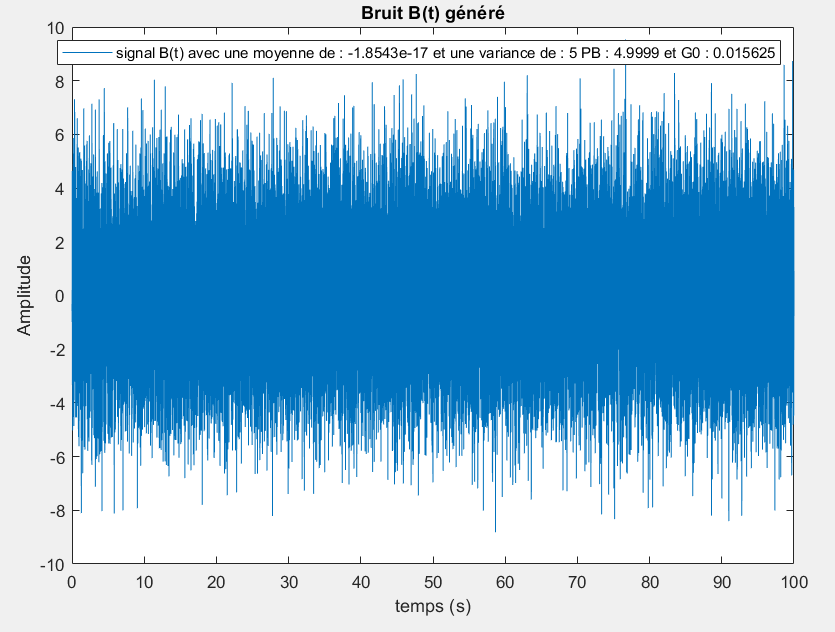
\includegraphics[width=0.7\textwidth]{images/bruitgenere.png}}
\caption{Réalisation du bruit avec la légende contenant la moyenne, l'écart-type, $\Gamma0$ empirique.}
\label{fig-B}
\end{figure}

\begin{figure}
\centerline{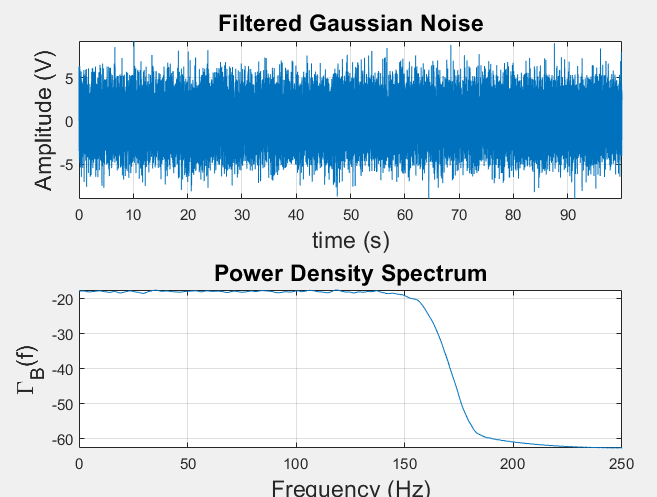
\includegraphics[width=0.7\textwidth]{images/bruitgen_G.png}}
\caption{Réalisation et densité spectrale de puissance moyenne  du bruit: $B=160~Hz$, $P_B= 5~V^2$, $\sigma_B = \sqrt{5}$, $\mu_B=0$.}
\label{fig-B}
\end{figure}
\newpage

\begin{table}[h]
\begin{center}
\begin{tabular}{| L{40mm} | C{40mm}|}\hline
Moyenne $B(t)$ 	& {$-1.8543 * 10^-17$}  	\\[5mm] \hline
Variance $B(t)$ & {$5$}   	\\[5mm] \hline
\end{tabular}
\end{center}
\label{table-B}
\caption{Mesures de la moyenne et de la variance de $B(t)$.}
\label{tab-B}
\end{table}

A partir  de la Figure \ref{fig-B} et en expliquant la démarche suivie, retrouver (approximativement) la valeur de $\Gamma_0$. Comparer à la valeur théorique de la préparation.\\
\newline
Dans la préparation, nous avons établi que le $\Gamma_0$ théorique vaut -18dB. Pour retrouver la valeur $\Gamma_0$ empirique, nous avons appliqué deux méthodes qui sont : 
\begin{itemize}
    \item  Méthode graphique : le $\Gamma_0$ correspond à la valeurs moyenne dans l'intervalle 0 à B (160 Hz). Sur la figure 2, nous observons que nous somme à un $\Gamma_0$ d'environ -18dB. 
    \item  Méthode de calcul empirique : nous pouvons calculer la Densité Spectrale de Puissance Moyenne (DSPM) à l'aide de la méthode des trapèzes et obtenir $\Gamma_0$ en divisant la DSPM par 2 fois la Bande passante. On obtient 0,01526, si l'on applique : $\Gamma_0 = 20*log(resultat)$ soit environ -18.063 dB.  
\end{itemize}
Nous pouvons en déduire que les valeurs empiriques sont cohérentes avec les valeurs théorique.
\newpage

\subsection{Etude du filtre passe-bande $\mathcal{F}_1$}
\label{sec:bruit-passe-bande}

On filtre le bruit $B(t)$ par un filtre passe-bande, de bande passante  $\Delta\nu$ centrée sur  la fréquence  $F_0$. 

\subsubsection{}

On choisit $\Delta\nu = \dnu~Hz$ et la valeur de $F_0$ identifiée dans la préparation.  \\
Reproduire dans le cadre ci-dessous, le code permettant de:
\begin{list}{-}{\setlength{\leftmargin}{3mm} \setlength{\labelwidth}{20mm} \setlength{\labelsep}{2mm} \setlength{\itemsep}{1mm} }
\item synthétiser le filtre $\mathcal{F}_1$ correspondant
\item filtrer le bruit $B(t)$ par le filtre $\mathcal{F}_1$ (afficher avec des légendes pertinentes, la sortie du {\tt BPF.m} dans la Figure \ref{fig-Y}) 
\item de mesurer sur la trace en sortie du filtre $\mathcal{F}_1$ les valeurs des paramètres demandés au Tableau 2:
\end{list}
\newline
Pour réaliser le filtre, nous avons utilisé la fonction \textit{BPF} (disponible sur CPe-Campus). Cette fonction génère une structure du signal filtré en fonction de 2 structures, la première qui est le bruit généré partie 1. La seconde partie est une structure contenant entier pour la fréquence d'échantillonnage, un entier pour la fréquence nu0, un entier pour le $\Delta_v$ et un entier pour l'ordre du filtre.  
\begin{verbatim}
% --- initialisaitons des variables
v0 = 100;
delta_v = 16;

% --- Création et filtrages s
Fp = struct('Fs',fs,'F0',v0,'Dnu',delta_v,'order',6,'class','BP filter') ;  
Y = BPF(X,Fp) ;

% --- Calculs des variables utiles
moyennedeBF = mean(Y.data);
variancedeBF = (std(Y.data))^2;
P_B_Y = trapz(Y.time,(Y.data).^2)/tmax;
Gamma_Y = P_B_Y/(2*b);
\end{verbatim}



\begin{figure}[h]
 \centerline{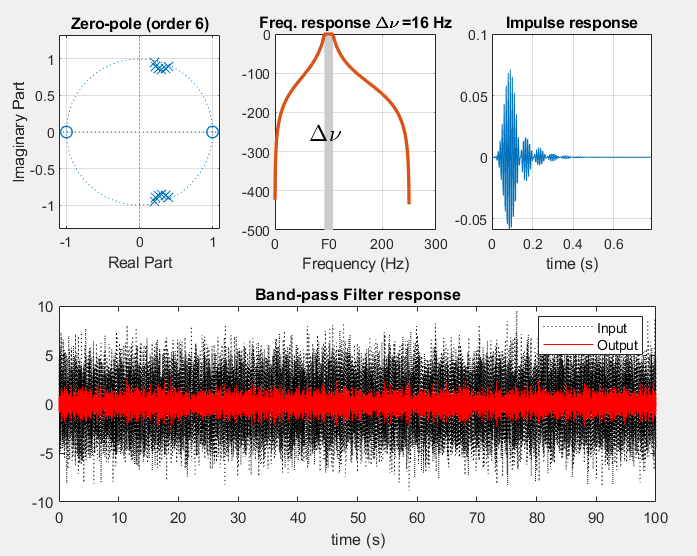
\includegraphics[width=0.7\textwidth]{images/filtreinit.png}}
 \caption{Bruit Y(t) filtré passe-bande pour $\Delta\nu = \dnu$ Hz}
 \label{fig-Y}
\end{figure}

\begin{figure}[h]
 \centerline{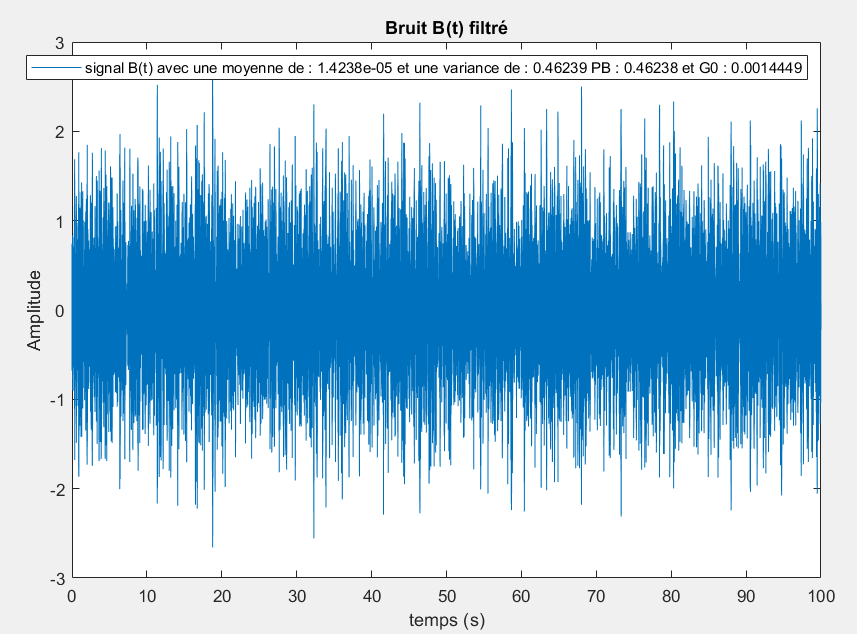
\includegraphics[width=0.7\textwidth]{images/bruitfiltre.png}}
 \caption{Bruit Y(t) filtré passe-bande pour $\Delta\nu = \dnu$ Hz}
 \label{fig-Y}
\end{figure}

\newpage
\begin{table}[t]
\begin{center}
\begin{tabular}{| L{40mm} | C{40mm}|}\hline
Moyenne $Y_{B}(t)$ 	& { 0 } 	\\[5mm] \hline
Variance $Y_{B}(t)$ &{ 0.46239 }   	\\[5mm] \hline
\end{tabular}
\end{center}
\caption{Mesures de la moyenne et de la variance de $Y_{B}(t)$.}
\label{table-YB}
\end{table}

\subsubsection{}

Estimer la valeur de $\Gamma_0$. Comparer les mesures ($\overline{P}_{Y_B}$ et $\Gamma_0$) aux valeurs théoriques obtenues en préparation. Comment peut on expliquer les éventuelles différence?\\
\newline
Dans la préparation, nous avons établi que le $PB$ théorique vaut 0.5, or la valeur $PB$ empirique est 0.4623 donc on obtient une variation d'environ 0.04. Cette variation peut être expliquer par l'utilisation de réalisation aléatoire empirique qui entraîne une variation sur les paramètres. Le $\Gamma_0$ empirique est de 0.001449 or la valeur $\Gamma_0$ théorique vaut 0.015 donc le filtre entraine aussi une variation sur la DSPM.  

\subsubsection{}
En pratique, qu'est ce qui limite le choix d'une  bande passante $\Delta \nu$ trop étroite ?\\
\newline
A l'aide de la relation entre temps et fréquence, si nous prenons une bande passante très étroites alors la réponse impulsionelle sera lente. Ainsi, il faut trouver un compromis en fonction du cahier des charges.   

\newpage
\subsection{Elévation au carré et Filtrage RC passe-bas}
\subsubsection{}

Comme précédemment, on choisit $\Delta\nu = \dnu Hz$. En faisant varier le produit $\Delta \nu \times RC$ dans une boucle (du type {\tt for \ldots end}), donner dans le cadre ci-dessous, le code qui:

\begin{list}{-}{\setlength{\leftmargin}{3mm} \setlength{\labelwidth}{20mm} \setlength{\labelsep}{2mm} \setlength{\itemsep}{1mm} }
\item génère le signal $Z_B(t)= Y_B^2(t)$ 
\item calcule la valeur de la constante $RC$ correspondant au produit $\Delta\nu \times RC$ choisi
\item filtre le signal $Z_B(t)$ par le filtre $\mathcal{H}_{I}$ de constante de temps $RC$  
\item mesure sur la sortie $W_B(t)$ les paramètres demandés dans la  Table \ref{table-WB}
\end{list}

\begin{verbatim}
% --- initialisaitons des variables
RC = 0;
tab_RC_dV = [2 20 100];
tab_Wb = [];
tab_RCP = [];

% --- Passage du signal dans le Quadrateur
Z_b = SquareSig(Y);

% --- Boucles de traitements des 3 cas
for i=1:3
    figure(3+i)
    % --- Calcul de la valeur RC en fonction du produit
    RC_dV = tab_RC_dV(i);
    RC = RC_dV/delta_v;
    % --- initialisaitons de la structure en fonction
    RCFp = struct('Fs',fs,'RC',RC);
    [Wb,RCFp] = RCF(Z_b,RCFp);
    tab_Wb = [tab_Wb; Wb];
    tab_RCP = [tab_RCP; RCFp];
end
\end{verbatim}


Remplir le tableau de mesures de la Table \ref{table-WB} (ignorez dans un premier temps les mesures demandées {\em après correction}).

\begin{table}[h]
\begin{tabular}{| L{40mm} | C{35mm} | C{35mm} | C{35mm} |}\hline
$\Delta\nu \times RC$ & 2 & 20 & 100 \\[5mm]  \hline\hline
$RC$ & 1/8  & 5/4 & 6.25 \\[5mm]  \hline \hline
moyenne $W_B(t)$  & 0.46185	& 0.4558	& 0.43242 	 	 \\[5mm] \hline
variance $W_B(t)$ 	& 0.4528	& 0.0059138	&	0.0060582 \\[5mm]  \hline
Kurtosis $W_B(t)$ 	& 5.3958 	& 6.6982	& 14.0553 \\[5mm]  \hline \hline
moyenne $W_B(t)$ \newline (après correction) 	& 0.4628	&	0.4605 & 0.45574	\\[5mm] \hline
variance $W_B(t)$ \newline (après correction) 		& 0.4628	& 0.0046886	&	 0.0039945\\[5mm]  \hline
Kurtosis $W_B(t)$  \newline (après correction)		& 5.4117	& 2.9536	&	2.36328 \\[5mm]  \hline
\end{tabular}
\caption{Sortie Filtre $RC$ - Cas du bruit seul.}
\label{table-WB}
\end{table}

\subsubsection{}
Le processus $Z_B(t)$ (\textbf{signal en sortie du quadrateur}) est-il gaussien? Pourquoi?\\
\newline
Nous étudions un processus aléatoire qui est un un bruit Gaussien centré généré à partir de la fonction \textit{rand}. Ce processus est filtré par un filtre linéaire et passé dans le Quadrateur, or aucun des deux éléments altère la nature du signal. Donc on observe un processus Gaussien.
\subsubsection{}
Pour les 2 valeurs extrêmes de $\Delta\nu \times RC$ proposées dans la Table \ref{table-WB}, afficher dans la Figure ci-dessous, les sorties de {\tt RCF.m}.

\begin{figure}[h]
\begin{tabular}{cc}
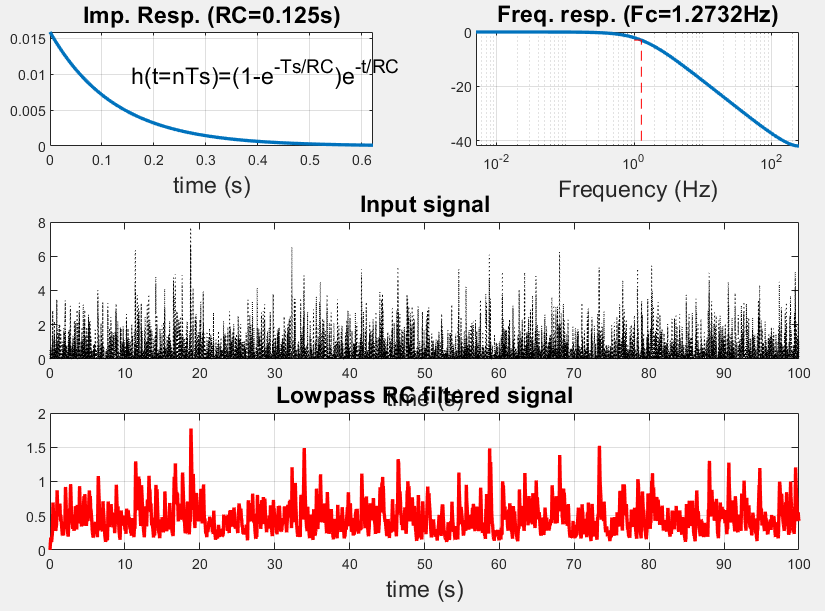
\includegraphics[width=0.5\textwidth]{images/rc_1.PNG} & 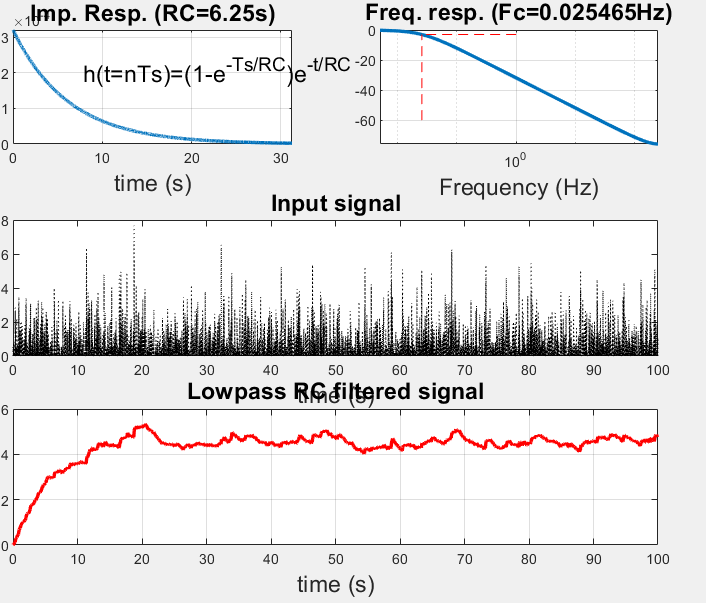
\includegraphics[width=0.5\textwidth]{images/rc_3.png} \\
\end{tabular}
 \caption{Sortie $W_B(t)$ du filtre passe-bas pour $\Delta\nu = 16$ Hz -- 
  (a) $RC$ = 1/8. ($\Delta\nu\times RC=2 $) (b) $RC = 6.25 $ ($\Delta\nu\times RC = 100 $) }
 \label{fig-Wb}
\end{figure}

\subsubsection{}

Comparer pour chaque valeur de la constante $RC$, la valeur moyenne mesurée à la valeur théorique déterminée dans la préparation. Qu'est ce qui peut expliquer ces différences? Comment corriger cet effet?  \\
\newline
Nous possédons un régime transitoire sur le filtre RC qui impacte les premières valeurs et qui biaises les indicateurs tel que la moyenne ou le Kurtosis.Ce régime dure environ 5 tau, donc on doit atteindre le régime permanent avant de mesurer les indicateurs. Cela se traduit en MATLAB  par ignorer les \textit{n} valuers pour n correspodnat 5 tau des vecteurs datas et time de la structure Z.

\subsubsection{}
Donner dans l'encadré ci-dessous les 2 lignes de code qui implémentent cette solution.

\begin{verbatim}
% --- Le premier indice > 5*tau
itrue = Wb.time >= 5*RCp.RC;

% --- Calcul des divers indicateurs
moyenne = mean(Wb.data(itrue));
variance = (std(Wb.data(itrue))).^2;
kurtosi = kurtosis(Wb.data(itrue));
\end{verbatim}

Appliquer cette correction et porter les nouvelles mesures dans la Table \ref{table-WB} (partie {\em avec correction}).


\subsubsection{}
Lorsque le Kurtosis est proche de $3$, que peut on dire de la statistique du processus $W_B(t)$? \\
\textbf{Quel théorème important ce résultat illustre-t-il?}\\
 Pour quelles(s) valeur(s) de $RC$ a-t-on une {\em intégration forte}?  Comparer les variances de $W_B(t)$ mesurées pour les deux valeurs extrêmes de $RC$. \\
\newline
Ces résultats illustrent le théorème Centrale Limite. Dans le cas d'un processus Gaussien, la valeur du Kurtosis est à 3. Pour étudier la valeur du Kurtosis rigoureusement, il faudrait réaliser un grand nombre fois le processus aléatoire et étudier la moyenne des valeurs obtenues car la valeur Kurtosis d'un processus aléatoire varie à chaque réalisation . 
\newline
L'intégration forte est l'approximation que les éléments portes et triangles autours de $\delta = 0$ sont très large et constant devant le module carrée de H(v). Pour assurer cette hypothèse il faut que $1/RC << \Delta_V$.
\newline
Dans notre cas, une simple étude d'une valeur suffit à déduire que les processus sont Gaussiens pour les valeurs 5/4 et 6.25 de RC, nous pouvons en déduire que plus le résultat $\Delta_v$*RC est important et plus le processus sera proche d'un processus Gaussien. 
\newline

\textbf{Dans la suite du TP, il faudra systématiquement appliquer cette correction aux mesures effectuées en sortie du filtre RC.}

\clearpage
\section{Mélange Signal + Bruit}
\label{sec:melange}

On étudie à présent le signal $W(t)$ en sortie du filtre RC passe-bas, lorsque le mélange $X(t) = S(t) + B(t)$ est reçu en entrée du détecteur.

\subsection{Sortie du filtre passe-bande $\mathcal{F}_1$}

\subsubsection{}

En utilisant  les paramètres déterminés en préparation, générer une réalisation du signal $S(t)$ sur la même durée $T=100~s$ et la même fréquence d'échantillonnage $F_s = 500~Hz$. \\[1mm]
Reporter le code correspondant ci-dessous.

\debutrep{code ci-dessous}
\begin{verbatim}

\end{verbatim}
\finrep

 
\subsubsection{}

Vérifier que le filtre passe-bande, s'il est accordé sur la fréquence $\nu_0$ n'altère pas le  signal $S(t)$, en mesurant en sortie de $\mathcal{F}_1$ (dans le cas où $S(t)$ se présente seul en entrée) les paramètres demandés à la Table \ref{table-YSB}. En reprenant les mesures  effectuées au paragraphe \ref{sec:bruit-passe-bande}, déterminer le rapport signal sur bruit $\eta_{E_1}$ en sortie du sortie du filtre $\mathcal{F}_1$ ainsi que le gain $\eta_{E_1}/\eta_E$ introduit par $\mathcal{F}_1$.


\begin{table}[h]
\begin{center}
\begin{tabular}{| L{40mm} | C{40mm}|}\hline
Fréquence $Y_{S}(t)$ 		&  	\\[5mm] \hline
Amplitude $Y_{S}(t)$ 		&  	\\[5mm] \hline
Puissance  $Y_{S}(t)$ 		&  	\\[5mm] \hline
Puissance  $Y_{B}(t)$  \newline
(recopie Table \ref{table-YB}) &  	\\[5mm] \hline
SNR $\eta_{E_1}$ 		& 	\\[5mm] \hline
Gain $\eta_{E_1}/\eta_E$ 	& 	\\[5mm] \hline
\end{tabular}
\end{center}
\caption{Mesures des SNR et gains en sortie de $\mathcal{F}_1$.}
\label{table-YSB}
\end{table}

\subsubsection{}

Comparer aux valeurs théoriques.

\debutrep{réponse ci-dessous}

\finrep

\subsection{Sortie du filtre RC passe-bas}

\subsubsection{}

Dans les mêmes conditions expérimentales  ($\overline{P_B} = 5~V^2$,  $\Delta\nu = \dnu Hz$, $\eta_E=-10~dB$), effectuer les différentes mesures demandées dans le tableau \ref{table-WSB}. 

\begin{table}
\begin{tabular}{|L{6mm}| L{40mm} | C{35mm} | C{35mm} | C{35mm} |}\hline
	& $\Delta\nu \times RC$ 		& 2 	& 20 	& 100 \\[5mm]  \hline
	& $RC$ 					& 	&	&	\\[5mm]  \hline \hline
T	& $S_S$ 					&	&	&	\\[5mm]  \cline{2-5} % \hline
H	& $B_S=\mathbb{S}td\{W_{S+B}\}$ &	&	&	\\[5mm]  \cline{2-5} %  \hline
É	& SNR $\eta_S$				&	&	&	\\[5mm]  \cline{2-5} %  \hline 
O	& Gain $g_1$				&	& 	&	\\[5mm] \cline{2-5} % \hline
. 	& Gain $g$ 				&	&	&	\\[5mm]  \hline\hline
M 	& moyenne $W_B$ \newline 
(recopie de Table \ref{table-WB}) 		&	&	&	\\[5mm]  \cline{2-5} %\hline
E 	& moyenne $W_{S+B}$  		&	&	& 	\\[5mm]  \cline{2-5} %\hline
S 	& $S_S$ 					&	&	&	\\[5mm]  \cline{2-5} %\hline
U 	& $B_S=\mathbb{S}td\{W_{S+B}\}$ &	&	&	\\[5mm]  \cline{2-5} % \hline
R 	& SNR $\eta_S$ 				&	&	&	\\[5mm]  \cline{2-5} % \hline 
E 	& Gain $g_1$ 				&	&	&	\\[5mm]  \cline{2-5} %\hline
S 	& Gain $g$ 				&	&	&	\\[5mm]  \hline\hline
\end{tabular}
\caption{Sortie Filtre $RC$ - Cas du mélange signal $+$ bruit.}
\label{table-WSB}
\end{table}


\subsubsection{}

Représentez dans la Figure \ref{fig-Wsb}, la sortie de {\tt RCF.m} correspondant au cas  $\Delta\nu \times RC = 20$.

\debutrep{figure ci-dessous}
\begin{figure}[h]

\caption{Signal $W_{S+B}(t)$ dans le cas du mélange signal + bruit ($\Delta \nu = 16$ Hz, $\Delta\nu \times RC = 20$)}
\label{fig-Wsb}
\end{figure}
\finrep

\clearpage

\section{Transmission d'un message binaire}

\subsection{Modulation binaire périodique}

On souhaite à présent transmettre et détecter une séquence périodique binaire.\\

\subsubsection{}

Avec les paramètres suivant:\\[-3mm]
\begin{list}{-}{\setlength{\leftmargin}{3mm} \setlength{\labelwidth}{20mm} \setlength{\labelsep}{2mm} \setlength{\itemsep}{1mm} }
\item[--] Puissance du bruit $B(t)$, $\overline{P}_{B}  = 5~V^2$
\item[--] Rapport signal sur bruit en entrée de la chaine, $\eta_E = -10~dB$
\item[--] Fréquence du signal modulant $M(t)$, $F_M = 0.05~Hz$
\item[--] Durée des signaux, $T = 100~s$\\[-2mm]
\end{list}

synthétiser les  signaux $S(t)$,  $B(t)$ et $X(t)$ correspondant. \\

En vous basant sur les résultats expérimentaux obtenus dans la partie \ref{sec:melange}, choisissez un jeu de paramètres pertinent pour calibrer les filtres 
$\mathcal{F}_1$ et $\mathcal{H}_I$. Reporter dans le cadre ci-dessous le code  de détection du signal binaire reçu. 

\debutrep{code ci-dessous}
\begin{verbatim}

\end{verbatim}
\finrep

\subsubsection{}

Visualiser dans la Figure \ref{fig-binaire}  (en organisant avec la commande {\tt subplot(4,1,$\cdot$)} et en ajoutant une légende pertinente), les signaux:\\[-3mm]
\begin{list}{-}{\setlength{\leftmargin}{3mm} \setlength{\labelwidth}{20mm} \setlength{\labelsep}{2mm} \setlength{\itemsep}{1mm} }
\item[--] $S(t)$
\item[--] $X(t)$
\item[--] $W(t)$
\item[--] Le signal binaire détecté obtenu par seuillage du signal $W(t)$ (commenter le choix du seuil $\Sigma$ choisi)
\end{list} 

\debutrep{figure ci-dessous}
\begin{figure}
\begin{tabular}{cc}
(a) & (b) \\
(c) & (d) \\
\end{tabular}
\caption{(a) Signal binaire $S(t)$. (b) Mélange Signal (binaire) + bruit avant et apres filtrage passe-bande. (c) Sortie $W(t)$ de la chaine de détection quadratique. (d) Signal binaire détecté après seuillage de la sortie quadratique.}
\label{fig-binaire}
\end{figure}
\finrep


\subsubsection{}

Indiquez les valeurs des paramètres de détection utilisés.

\debutrep{réponse ci-dessous}

\finrep

\subsubsection{}

Essentiellement quel élément de la chaine de détection va-t-il limiter le débit de transmission?

\debutrep{réponse ci-dessous}

\finrep

\subsubsection{}
Sans chercher à les estimer ici, quel(s) critère(s) permettrai(en)t de mesurer la qualité de la détection?

\debutrep{réponse ci-dessous}

\finrep


\subsection{Décodage d'un message inconnu}


Charger le signal reçu {\tt 'SignalRecu\_j'}, où $j$ est le numéro de votre binôme.\\[2mm]
{\tt >\!> load SignalRecu\_1}\\[2mm]
Le signal $X(t)$ correspond à un message codé (code ascii 7 bits) transmis par modulation d'amplitude et  dégradé par un bruit additif lié au canal de transmission. 
Exécuter  la  commande: \\[2mm]
{\tt >\!> [TxMsg,Xp] = RxMessage\_DQ(X,Xp) ; }  \\[2mm]
pour lancer une détection quadratique {\em automatique} sur le signal reçu $X$ (la structure $Xp$ contient tous les paramètres de la transmission).
Ajuster en ligne, les différents paramètres de la détection jusqu'à ce que le message décodé vous semble satisfaisant. Recopier ci-dessous, le message décodé. 

\debutrep{réponse ci-dessous}

\finrep


\section{Annexes}

\subsection{Evolution théorique du gain SNR ${\displaystyle g_1=\frac{\eta_s}{\eta_1}}$ en fonction de $\eta_1$ et de $RC \times \Delta\nu$}

\begin{center}
\includegraphics[width=0.9\columnwidth]{4ETI-TP-DQ-SNRgain.eps} 
\end{center}

\subsection{Documentation routines Matlab}
\label{sec:annexes-help}

\subsubsection{OOK.m}
   

        \color{lightgray} \begin{verbatim}  [S,Sp,M] = OOK(Sp)     Generates a ON-OFF keying modulated signal whose
  parameters are specified by the parameter structure Sp
  S(n) = M(n).A.cos(2.pi.Fc.n/Fs + phi)
  M(n) is either a binary periodic signal (0-1) oscillating at frequency FM
  or a 0-1 sequence defined by W (if specified W overides FM). OOK.m
  displays in the current window plot the synthesised signal.
 
  Inputs:
  Sp     signal structure containing the signal parameters with following fileds: 
            - Fs    sampling frequency of the signal (in Hz)
            - A     amplitude of the carrier
            - Fc    carrier frequency (in Hz)
            - FM    modulating frequency (0 = no modulation) (in Hz)
            - T     duration of the signal (in seconds)
            - W     binary word to be transmitted (overides periodic modulation)
            - Phi   initial phase of the carrier (r.v. unif dist. over (0,2\pi))
            - Class String defining the type of signal S
         If varargin is left empty, each field of 'Sp' is defined online
 
  Outputs:
  S     signal structure containing the synthesised OOK signal with fields:
            - data : 1-byN vector containing the data samples
            - time : 1-byN vector containing the time samples
            - Fs   : scalar indicating the sampling frequency
  
  Sp    parameter structure (same as input)
  M     signal structure containing the Modulant signal (same structure as S) 
    
 
  Example :
        Sp = struct('Fs',50e3,'A',2,'Fc',1e3,'FM',5e1,'Phi',0,'T',1e-1,'W',[])
        [S,Sp,M] = OOK(Sp) 
        plot(S.time,S.data,M.time,M.data,':r')
  or
        [S] = OOK() 
\end{verbatim} \color{black}


\subsubsection{CGN.m}

        \color{lightgray} \begin{verbatim}  [X,Xp] = CGN(Xp)  generates a filtered, centered, gaussian noise X
  according to the parameters specified in the parameter structure Xp
  CGN displays in the current window plot, the synthesised trace and the
  corresponding estimated power spectrum density. 
 
  Input
  Xp        parameter structure containg the follwoing fileds:
            - sigma : standard deviation
            - Fs    : scalar indicating the sampling frequency
            - B     : the bandwidth (in Hz, B < Fs/2)
            - T     : duration of the generated trace (in seconds)
         If varargin is left empty, each field of 'Xp' is defined online
 
  Outputs
  - X     signal structure with the following fields:
            - data : 1-byN vector containing the data samples
            - time : 1-byN vector containing the time samples
            - Fs   : scalar indicating the sampling frequency
  - Xp    parameter structure (same as input)
 
  Example
 
  Xp = struct('sigma',1,'Fs',1000,'B',200,'T',10) ;
  [X,Xp] = CGN(Xp) ;
  % or 
  [X,Xp] = CGN() ;
\end{verbatim} \color{black}
    


\subsubsection{AddSig.m}

        \color{lightgray} \begin{verbatim}  [S] = AddSig(X,Y) Computes the sum Z of the two signals X and Y.
 
  Inputs
  X, Y  Signal structures with fields:
            - data : 1-by-N vector containing the data samples
            - time : 1-by-N vector containing the time samples
            - Fs   : scalar indicating the sampling frequency
        X and Y must have same lenghths and same sampling frequencies
 
  Outputs
  Z      Signal structures with fields:
            - data : 1-by-N vector containing the data samples
            - time : 1-by-N vector containing the time samples
            - Fs   : scalar indicating the sampling frequency
\end{verbatim} \color{black}

\subsubsection{BPF.m}


        \color{lightgray} \begin{verbatim}  [Y,Fp] = BPF(X,Fp) filters the signal structure X with a digital band-pass filter whose 
  parameters are specified in the Fp structure.
  BPF diplays in a single window plot, the zero-pole diagram, the frequency 
  and the impulse responses of the filter, and superimposed, the input and
  the output signals.
 
  Inputs
  - X    input signal structure with the following fields:
            - data : 1-byN vector containing the data samples
            - time : 1-byN vector containing the time samples
            - Fs   : scalar indicating the sampling frequency
  - Fp   parameter structure with following fields:
            - Fs   : scalar indicating the sampling frequency (must be
            identical to that of X)
            - F0   : the central frequency (in Hz)
            - Dnu  : the bandwidth 
            - order : integer corresponding to the order of the filter 
            - class : text string indicating the type of the filter.
 
  Outputs
  - Y     output signal structure with the following fields:
            - data : 1-byN vector containing the data samples
            - time : 1-byN vector containing the time samples
            - Fs   : scalar indicating the sampling frequency
  - Fp   parameter structure (same as input)
 
  Example:
  Fp = struct('Fs',1000,'F0',100,'Dnu',32,'order',6,'class','BP filter') ;  
  [X,Xp] = CGN() ;
  Y = BPF(X,Fp) ;
\end{verbatim} \color{black}



\subsubsection{SquareSig.m}

        \color{black} \begin{verbatim}  [Y] = SquareSig(X)    Computes the square amplitude Y of signal X.
 
  Inputs
  X     Signal structure with fields:
            - data : 1-by-N vector containing the data samples
            - time : 1-by-N vector containing the time samples
            - Fs   : scalar indicating the sampling frequency
 
  Outputs
  Y      Signal structures with fields:
            - data : 1-by-N vector containing the data samples
            - time : 1-by-N vector containing the time samples
            - Fs   : scalar indicating the sampling frequency
 
  Example:
  X = OOK() ;
  Y = SquareSig(X) ;
\end{verbatim} \color{black}
    


\subsubsection{RCF.m}

        \color{lightgray} \begin{verbatim}  [Y,RCFp] = RCF (X,RCFp) filters the signal structure X with a digital lowpass RC filter whose 
  parameters are specified in the RCFp structure.
  The z-transform of a lowpass RC filter is equal to
  H(z) = B(z)/A(z) = (1-a) / (1 - a z^(-1)) 
  where a = exp(-T/RC), and T is the sampling period
  RCF diplays in a single window plot, respectively the time and the frequency responses
  of the filter, the input signal and the output signal.
 
  Inputs
  - X     input signal structure with the following fields:
            - data : 1-byN vector containing the data samples
            - time : 1-byN vector containing the time samples
            - Fs   : scalar indicating the sampling frequency
  - RCFp  parameter structure with following fields:
            - Fs   : scalar indicating the sampling frequency (must be
            identical to that of X)
            - RC   : scalar defining the time constant RC (must be larger
            than 1/Fs)
 
  Outputs
  - Y     output signal structure with the following fields:
            - data : 1-byN vector containing the data samples
            - time : 1-byN vector containing the time samples
            - Fs   : scalar indicating the sampling frequency
  - RCFp   parameter structure (same as input)
\end{verbatim} \color{black}


\subsubsection{RxMessage\_DQ.m}

        \color{lightgray} \begin{verbatim}  [RxMsg,Xp,RxBinMsg] = RxMessage_DQ(X,Xp)     performs a Quadratic
  Detection of binary message conveyed in signal structure X. Xp is a structure 
  that contains all parameters related to the transmission. X and Xp are
  usually the output of routine TxMessage
\end{verbatim} \color{black}



\end{document}
































